\subsection{Chain of Responsability}
\label{chain-of-responsability}

\textbf{Scopo}: Comportamentale \\
\textbf{Raggio d'azione}: Oggetti

\paragraph{Definizione} Il pattern Chain of Responsability permette di evitare l'accoppiamento di una richiesta del mittente e del destinatario, facendo in modo che entrambi riescano ad averla esaudita. Consente di passare le richieste lungo una catena di gestori. Dopo aver ricevuto una richiesta, ciascun gestore decide di elaborarla o di trasmetterla al gestore successivo nella catena.

\begin{figure}[H]
    \centering
    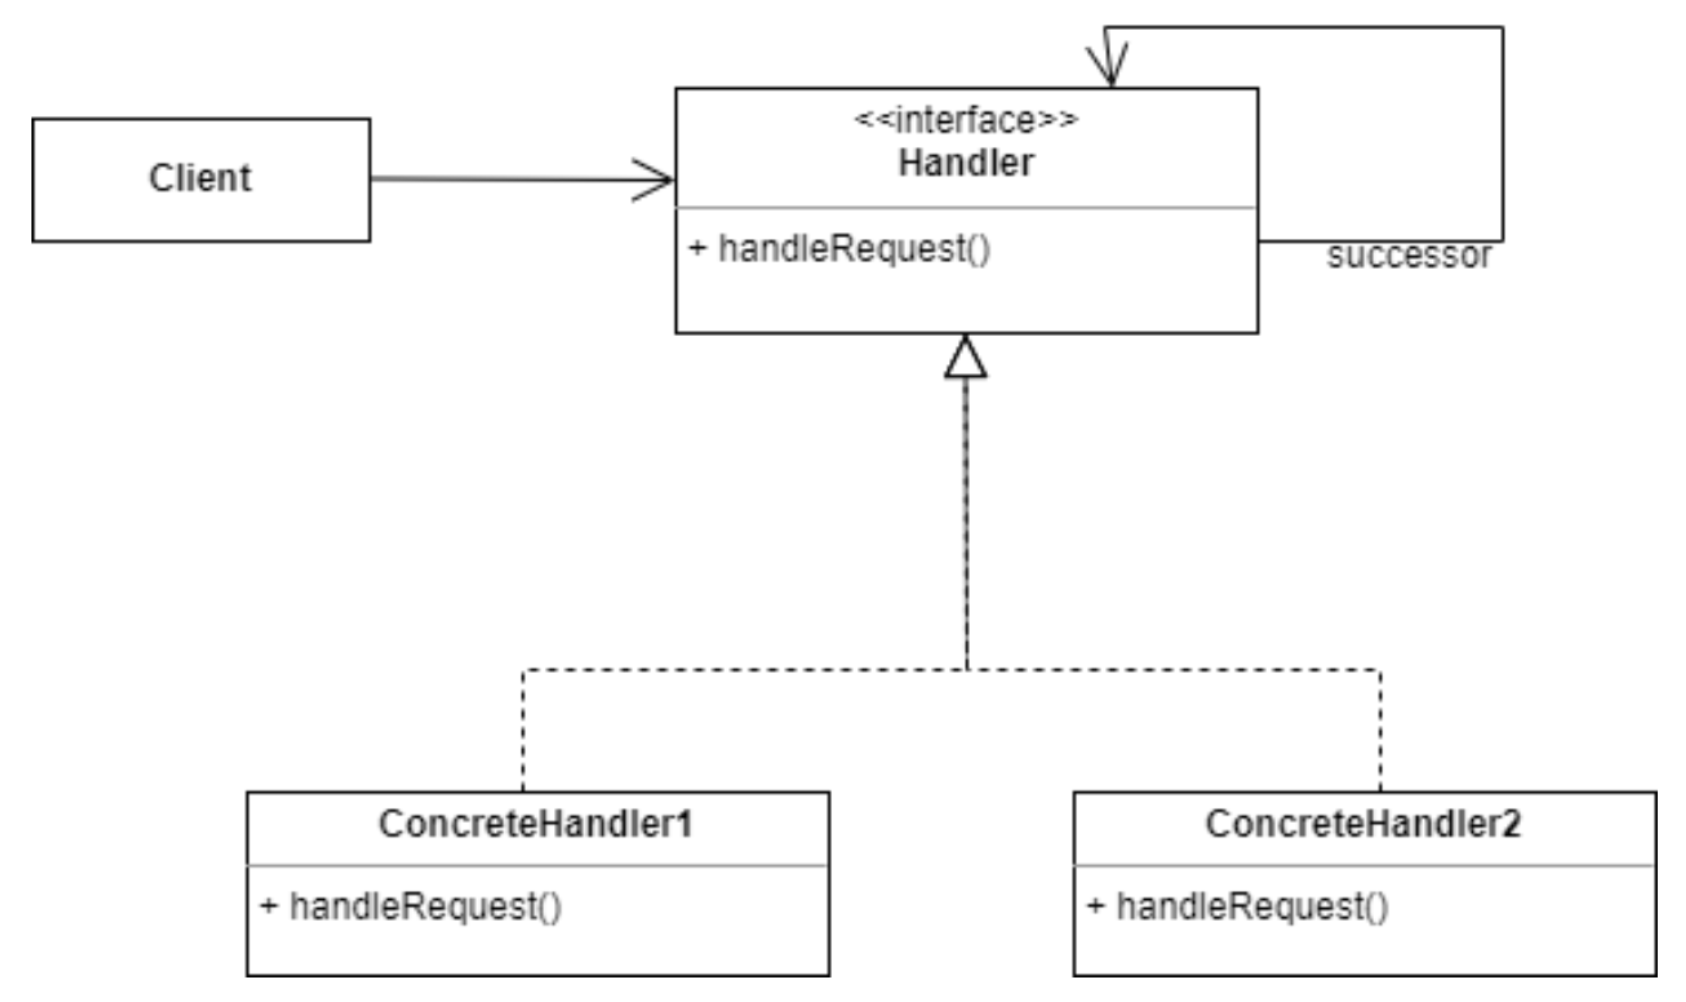
\includegraphics[width=0.4\linewidth]{assets/pattern/chain-of-responsability/cor-struttura.png}
    \caption{Struttura del pattern}
\end{figure}

\paragraph{Applicabilità} Il pattern CoR risulta utile quando si prevede che il programma elabori diversi tipi di richieste in vari modi, ma i tipi esatti di richieste e le relative sequenze sono sconosciuti in anticipo, quando è essenziale eseguire diversi gestori in un ordine particolare o quando si suppone che l'insieme di gestori e il relativo ordine cambino in fase di esecuzione.

CoR viene spesso utilizzata insieme a Composite (\ref{composite}). In questo caso, quando un componente foglia riceve una richiesta, può passarla attraverso la catena di tutti i componenti genitore fino alla radice dell'albero degli oggetti.

\begin{figure}[H]
    \centering
    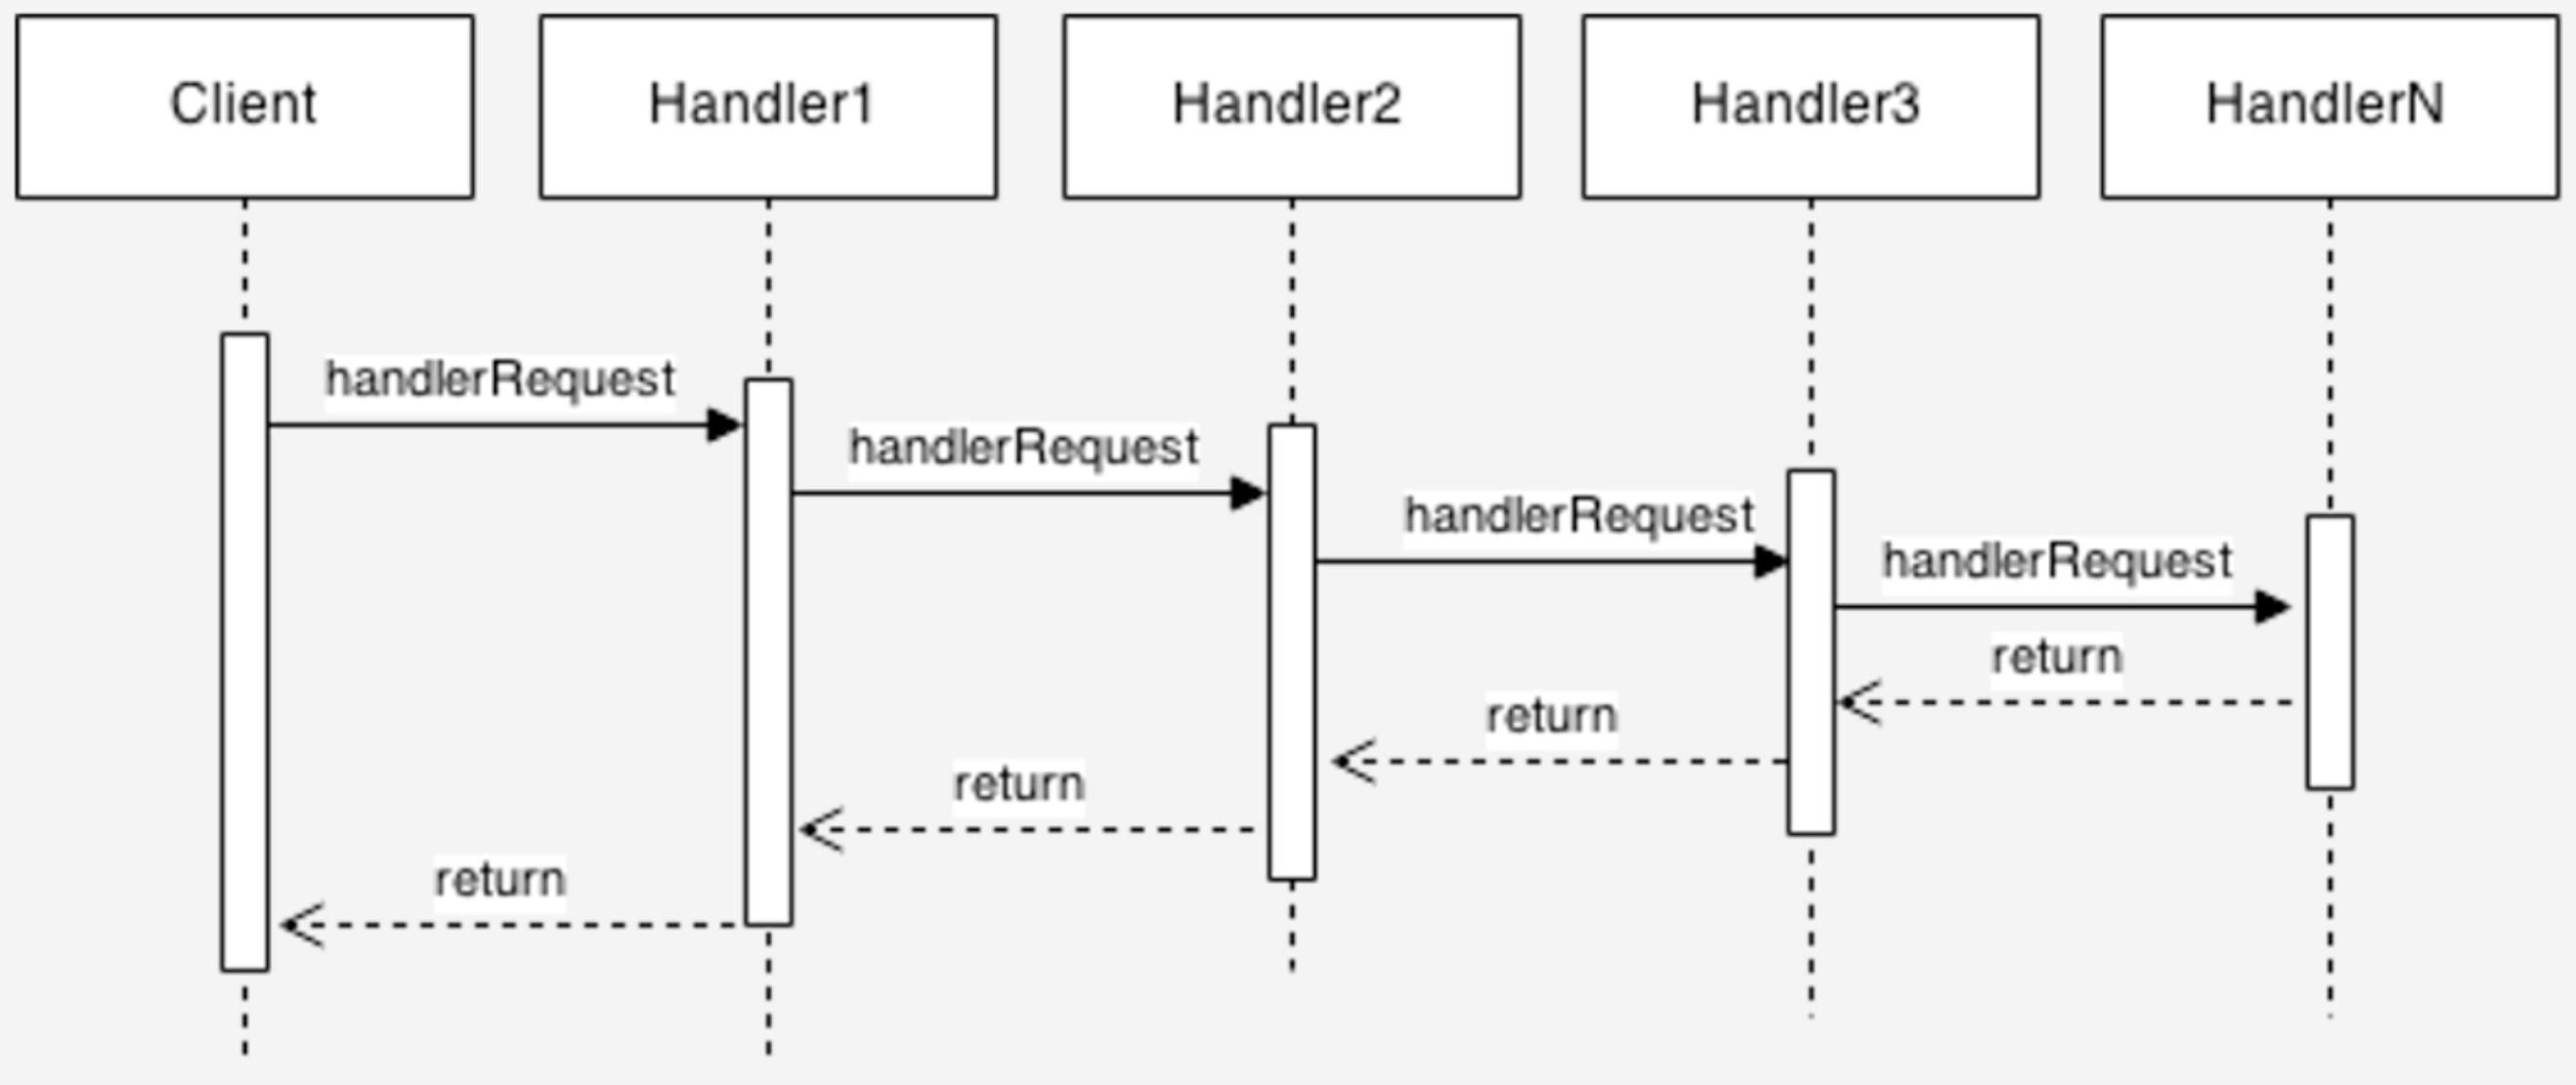
\includegraphics[width=0.8\linewidth]{assets/pattern/chain-of-responsability/cor-sequence.png}
    \caption{Sequence Diagram del patter Chain of Responsability}
\end{figure}

\newpage